%!TEX root = main.tex

\section{Numerical experiments} % (fold)
\label{sec:numerical_experiments}

\subsection{Setup}
the lbfgs is the one of scipy


\subsection{Analysing on toy problem}































\subsection{Integrating \emph{Screenkhorn} into machine learning pipelines}

In this subsection, we analyse the impact of using \emph{Screenkhorn}
instead of Sinkhorn in a complex machine learning pipeline. Our two applications
are a dimensionality reduction technique, denoted as Wasserstein Discriminant Analysis (WDA), based on Wasserstein distance approximated
through Sinkhorn divergence \cite{flamary2018WDA} and a domain-adaptation using optimal transport mapping \cite{courty2017optimal}, named OTDA. For both applications, we have based our code
on the ones of POT \cite{flamary2017pot} and just replaced the Sinkhorn function call with a Screenkhorn one.

WDA aims at finding a linear projection which minimize the ratio of distance between intra-class samples and distance inter-class samples, where the distance is understood
in a Sinkhorn divergence sense. We have considered the POT's default Sinkhorn stopping criterion parameters and for Screenkhorn, the LBFGS algorithm is stopped when the 
largest component of the projected gradient is smaller than $10^{-9}$, when the
number of iterations of number of objective function evaluations reach $10^{6}$.

Figure \ref{fig:wda} presents the gain in computational time we get as the number
of examples evolve and for different decimation factors of the \emph{Sinkhorn} problem.

\begin{figure*}[t]
	\centering
%	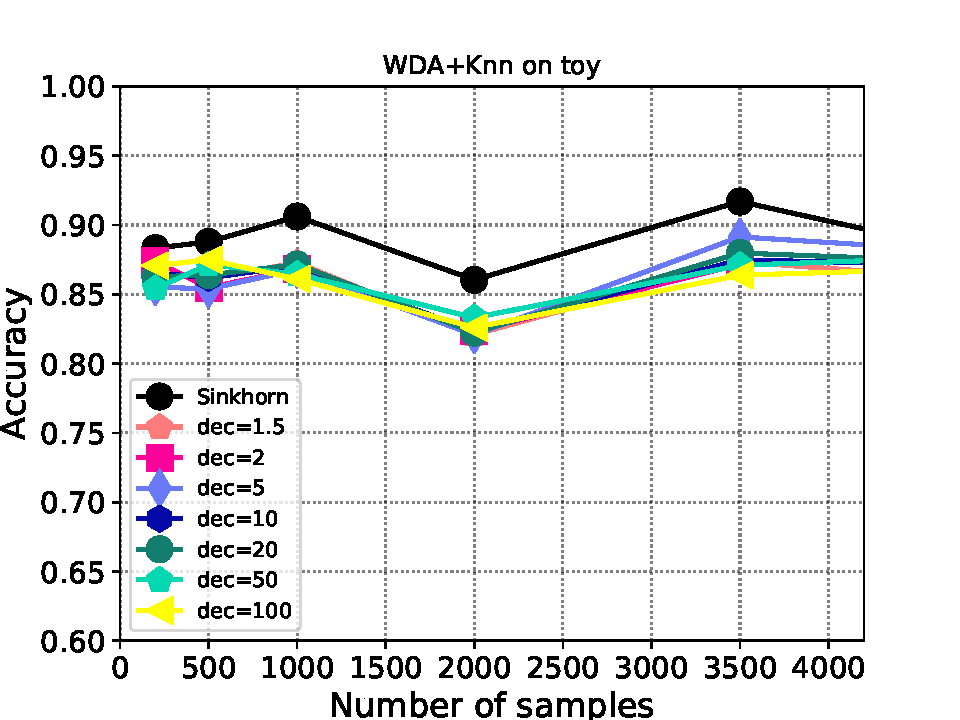
\includegraphics[width=4.cm]{../../figure/wda_accur_toy.pdf}
%	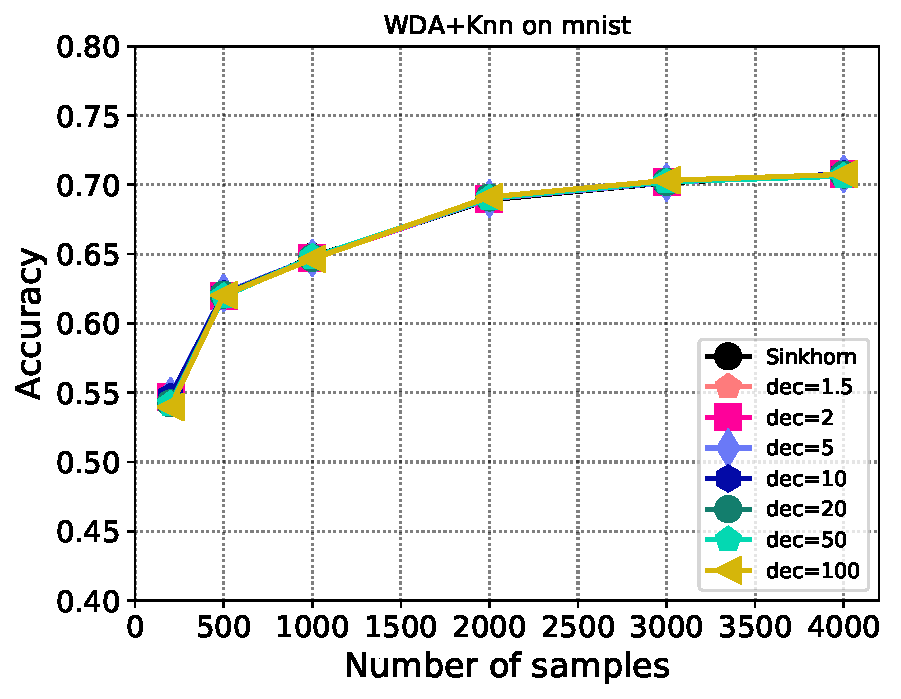
\includegraphics[width=4.cm]{../../figure/wda_accur_mnist.pdf}
	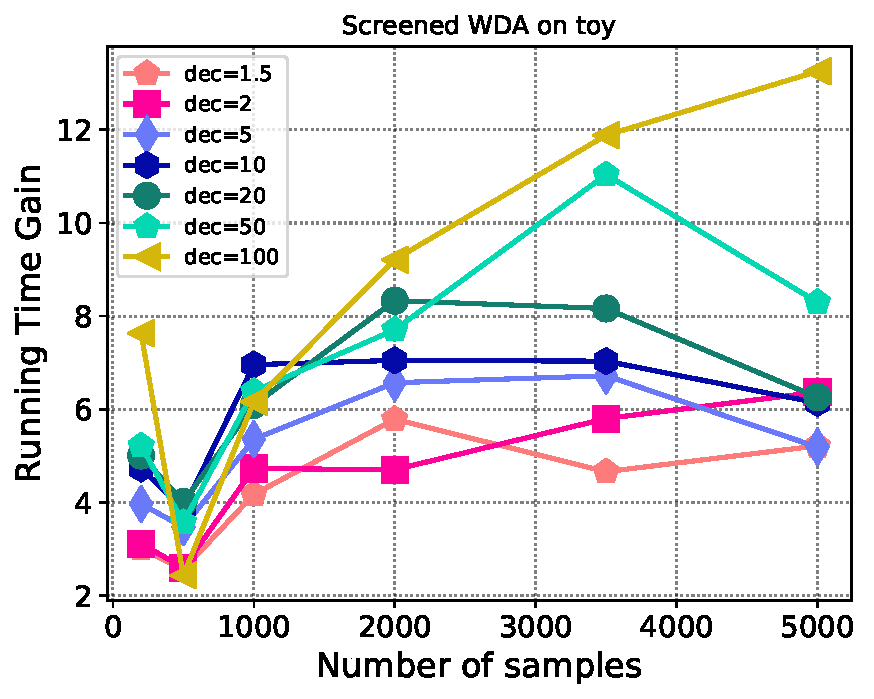
\includegraphics[width=6.cm]{../../figure/wda_gain_toy.pdf}
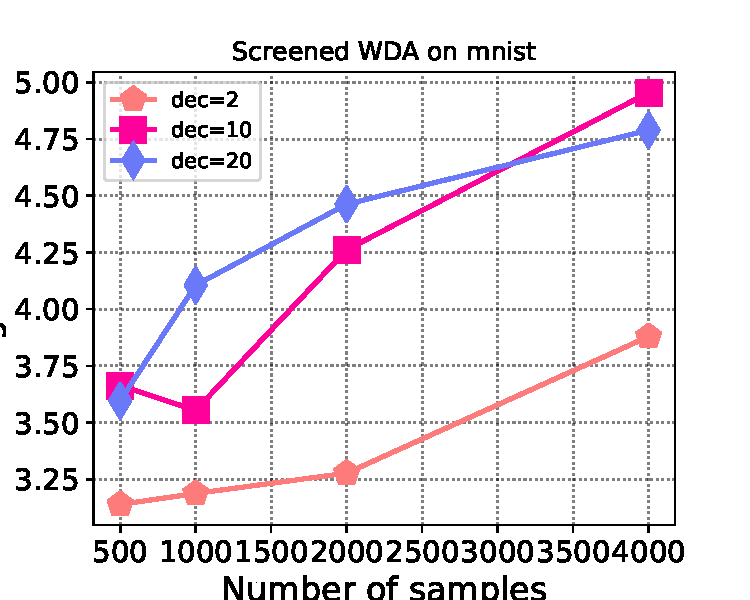
\includegraphics[width=6.cm]{../../figure/wda_gain_mnist.pdf}
	\caption{Wasserstein Discriminant Analysis : running time gain for a toy dataset and for mnist as a function of the number of examples and the data decimation factor in \emph{Screenkhorn}}.
	\label{fig:wda}
\end{figure*}
\begin{figure*}[t]
	\centering
	%	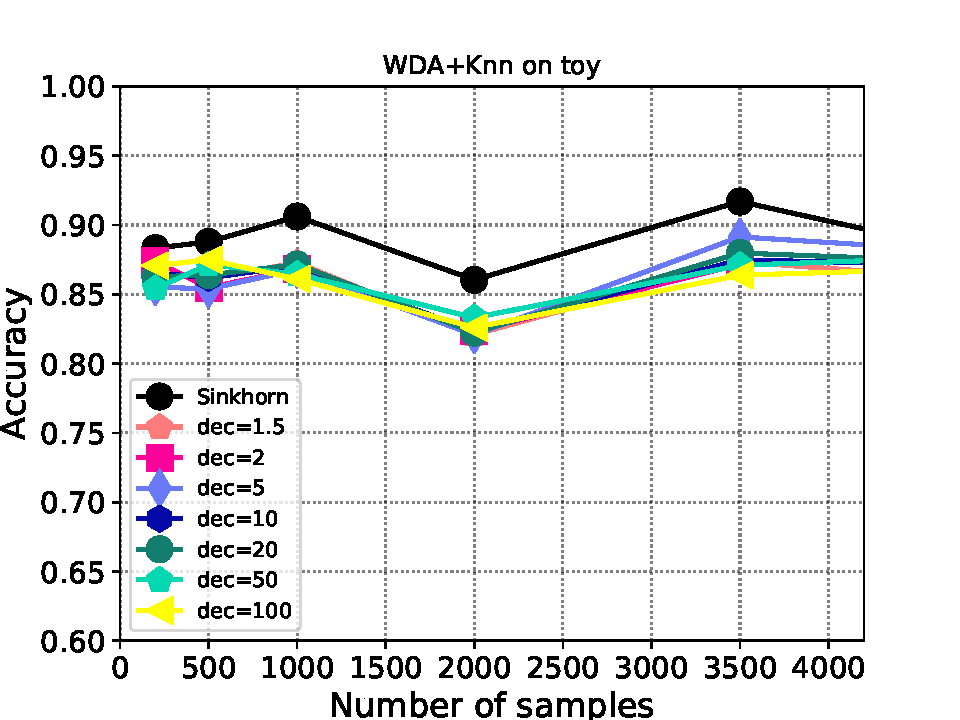
\includegraphics[width=4.cm]{../../figure/wda_accur_toy.pdf}
	%	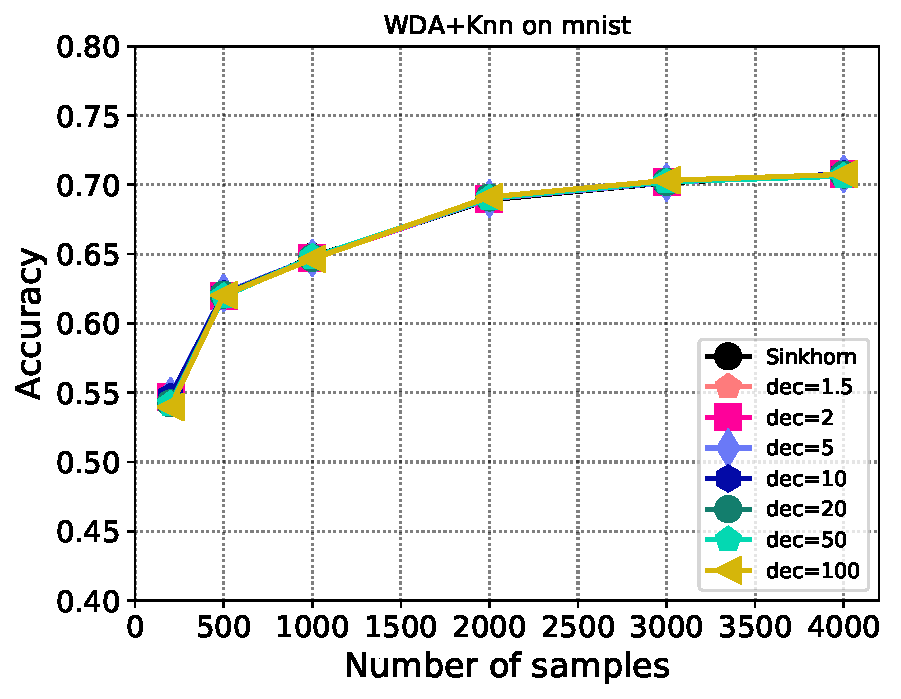
\includegraphics[width=4.cm]{../../figure/wda_accur_mnist.pdf}
	\includegraphics[width=6.cm]{../../figure/da_gain_toy.pdf}
	\includegraphics[width=6.cm]{../../figure/da_gain_mnist.pdf}
	\caption{OT Domain adaptation : running time gain for a toy dataset and for mnist as a function of the number of examples and the data decimation factor in \emph{Screenkhorn}}.
	\label{fig:otda}
\end{figure*}



% section numerical_experiments (end)